\chapter{Specifications}\label{sec:specifications}

The initial task of the project was to define the project goals and specifications, and the basic structure of the development plan.\\ 

Overall, the project aims to achieve a well-understood and demonstrable foundation for more independent Cublis, staying as true as possible to the following prerogatives:

\begin{itemize}

\item[] All original cubli capabilities are to be available through the augmented interface.

\item[] New capabilities are to be developped. As a result, Cublis are to autonomously carry out choreographies composed inside the augmented interface.

\item[] Choreographies are to be defined as several cublis performing a sequence of actions. These sequences can all be identical ( i.e. all cublis perform the same moves at the same time ), but it must also be possible to have each robot perform a different sequence.

\item[] Optimally Cublis are to communicate with each other as well as the computer, if that is not practical hierarchy can be imposed, with a leading cubli, or using the computer as the centralized node in communications.

\item[] Autonomy of choreographies is considered a positive aspect. That is, necessity of human intervention during a choreography should be as low as possible. On the other hand,  unexpected human intervention ( e.g. someone pushing a cubli over ) should be reasonably handled.

\end{itemize}




\section{Project Modules}

Thinking of the necessary components and the actions which would be required of them in order to generate the desired behavior, it was clear that at the minimum the project would require two separate programs, and thus at least two code bases. In addition, acting as a bridge within the two, and since it would likely be a quite significant endeavor in itself, the communication code was also separated conceptually and is discussed in the following as such.\\ 

 From this understanding, development is split into three main modules :

\begin{enumerate}
\item App behavior implementation - User Experience (C++)  
\item Communications implementation  (C++/C)
\item Cubli behavior implementation  (C)  
\end{enumerate}
 
Which can be described as follows:

\subsubsection{App Behavior Implementation}

The choreographer application has to be designed from scratch, providing an efficient and reliable way for users to interact wirelessly with the cubli. \\

One of the main objectives when designing the interface was for it to be as simple and intuitive as possible.
 
\subsubsection{Communications Implementation}

Acting as a bridge between the cubli and choreographer source code, the communications protocol behavior has to match in both cases, allowing messages encrypted in one to be decrypted by the other.

\begin{description}
\item[] Desired specifications for the protocol :
\begin{description}
  \item[Robust] - Ensuring that messages are transmitted successfully, and    strict prevention of information corruption in the process. 

  \item[Lightweight] - Minimal amount of processor overhead in order to not disrupt other tasks in cubli 

  \item[Concise] - Making messages as short as possible while ensuring that 	any information which needs to be transferred can be conveyed using the 	protocol. 

  \item[Cross-compatible] - Ensuring that the code could be compiled on the 	two other modules and would yield the same behavior (c.f. signedness 	issues) 
\end{description}
\end{description}
 
\subsubsection{Cubli Behavior Implementation}

Having received information representing the choreography description, status of other cubes, or user commands, the cubli has to react accordingly.

Pre-existing cubli source code had to be supplemented and modified to implement the expected behavior.




\subsection{Choreographer Application Specifications}

The goal is to create the choreographer application, an easy to launch and use executable.

Its specified core functionalities are:

\begin{itemize}
\item Choreography creation, and following that, modification
\item Choreography execution and control
\item Real-time display of choreography status
\item Real-time display of cubli status
\end{itemize}

along with the implied necessary functionalities:

\begin{itemize}
\item Communication with Cubli, and optionally display of those communications
\item Options for setting up the serial port
\end{itemize}


The application itself could in theory take many forms and still satisfy the necessary functionality. In order to decide which direction to take, examples of existing implementations were considered. These examples are applications with uses unrelated to the cubli choreographer, but which contain UI aspects that fulfill similar requirements as the ones pertaining to the choreographer application.\\

As an example, it would be possible to satisfy all those functionalities in a command-line interface ( \textit{c.f. Figure \ref{img:CommandLine}} ) . However, ease of use and simplicity go out the window in such an implementation when it comes to the timeline creation process. For that reason particularly, a graphical user interface, although it requires longer and more complex development, was deemed optimal.\\

\begin{figure}[ht]
   \centering
   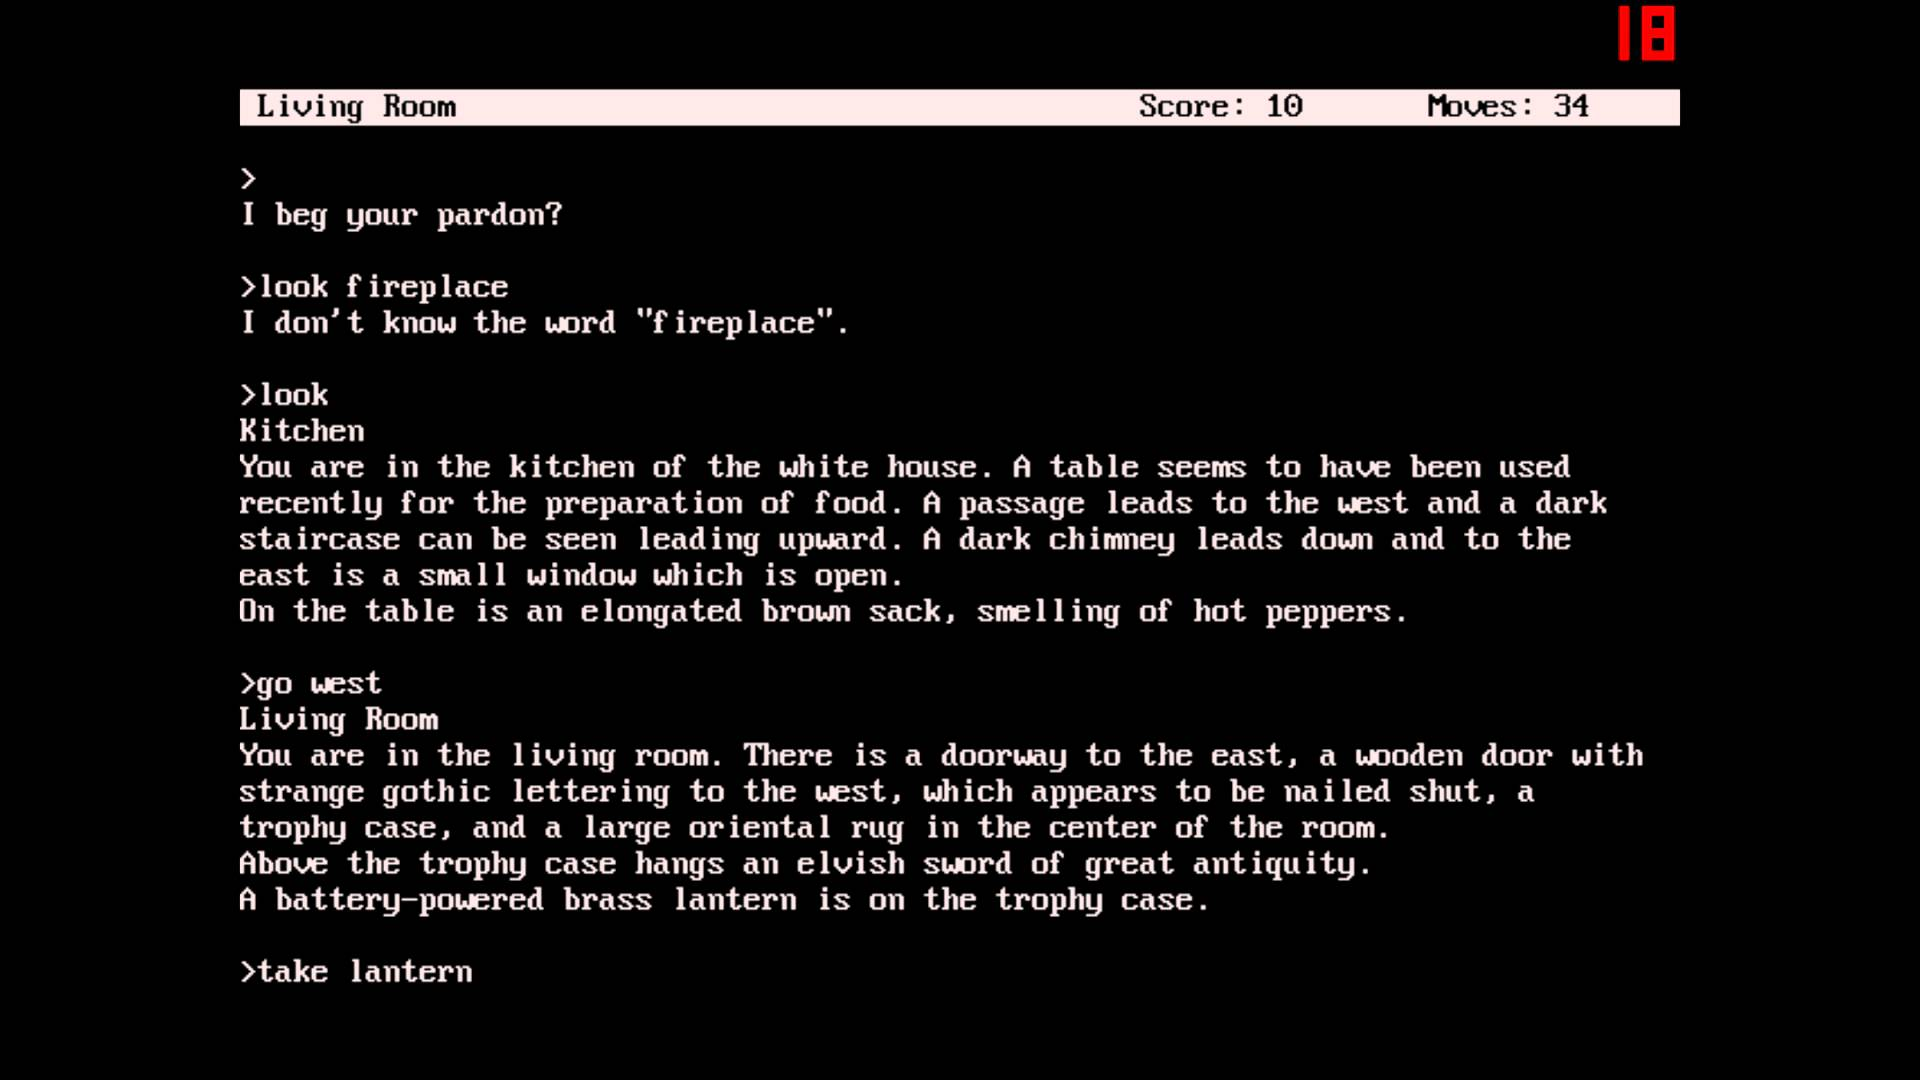
\includegraphics[width=0.75\textwidth]{img/CommandLine.jpg}
   \caption{Command-line interfaces can be used for many purposes.}
   \label{img:CommandLine}
\end{figure}

In fact, since the creation process lies at the center of the choreographer concept, and due to the other functionalities requiring little screen space in comparison, it makes sense for the choreography creation interface to occupy most of the interface, and dictate many design decisions.\\

Remaining functionalities to fulfill would be choreography control, port and application settings, extra user information and communication display.\\

In designing the interface, the parallel was made media music applications since the idea of a choreography can be conceptually tied with music. This applies in particular to the choreography control interface ( \textit{c.f. Figure \ref{img:GoogleMusic}} ).\\

\begin{figure}[ht]
   \centering
   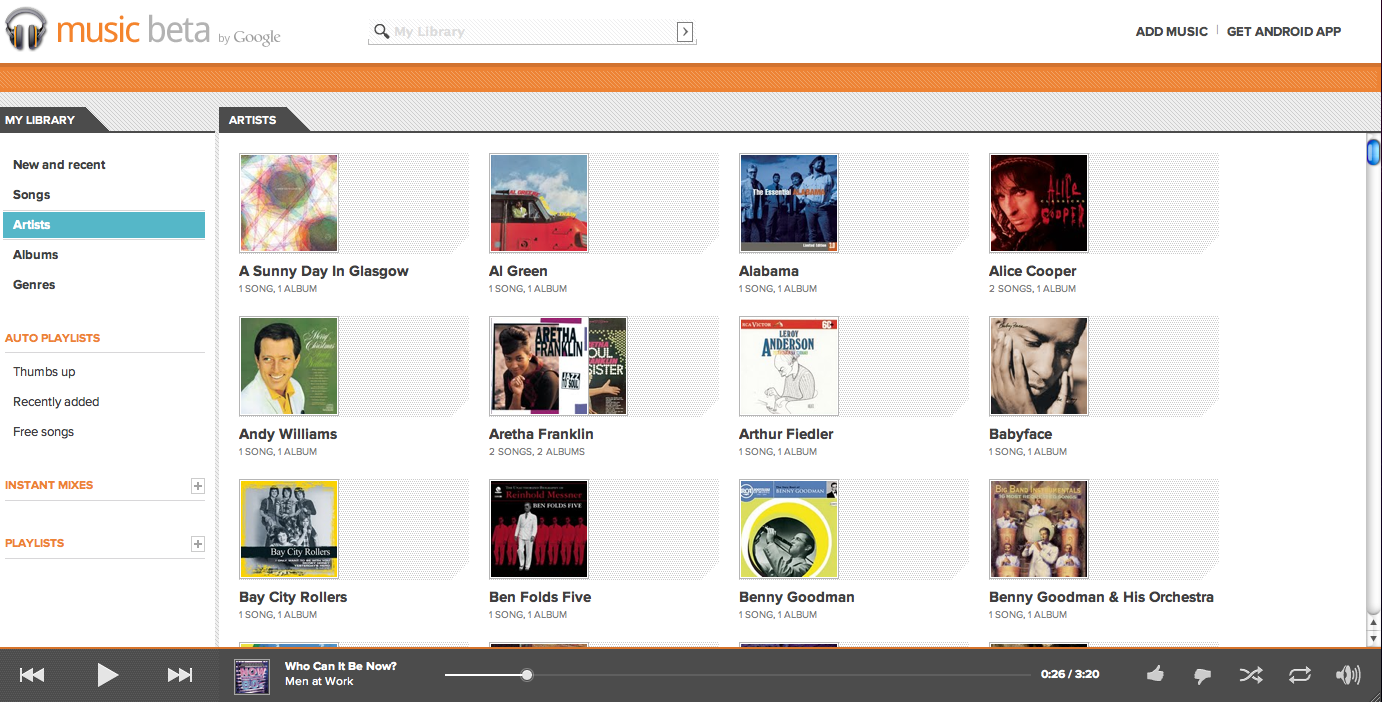
\includegraphics[width=0.75\textwidth]{img/GoogleMusic.png}
   \caption{Example of music player. Relevant are the simple controls at the bottom.}
   \label{img:GoogleMusic}
\end{figure}

In a similar vein, music or video creation/splicing softwares often deal with similar manipulation of time-dependent sequences by the user, and their solutions are particularly suited to the purposes of this project ( \textit{c.f. Figure \ref{img:MusicEditor}} ).\\

\begin{figure}[ht]
   \centering
   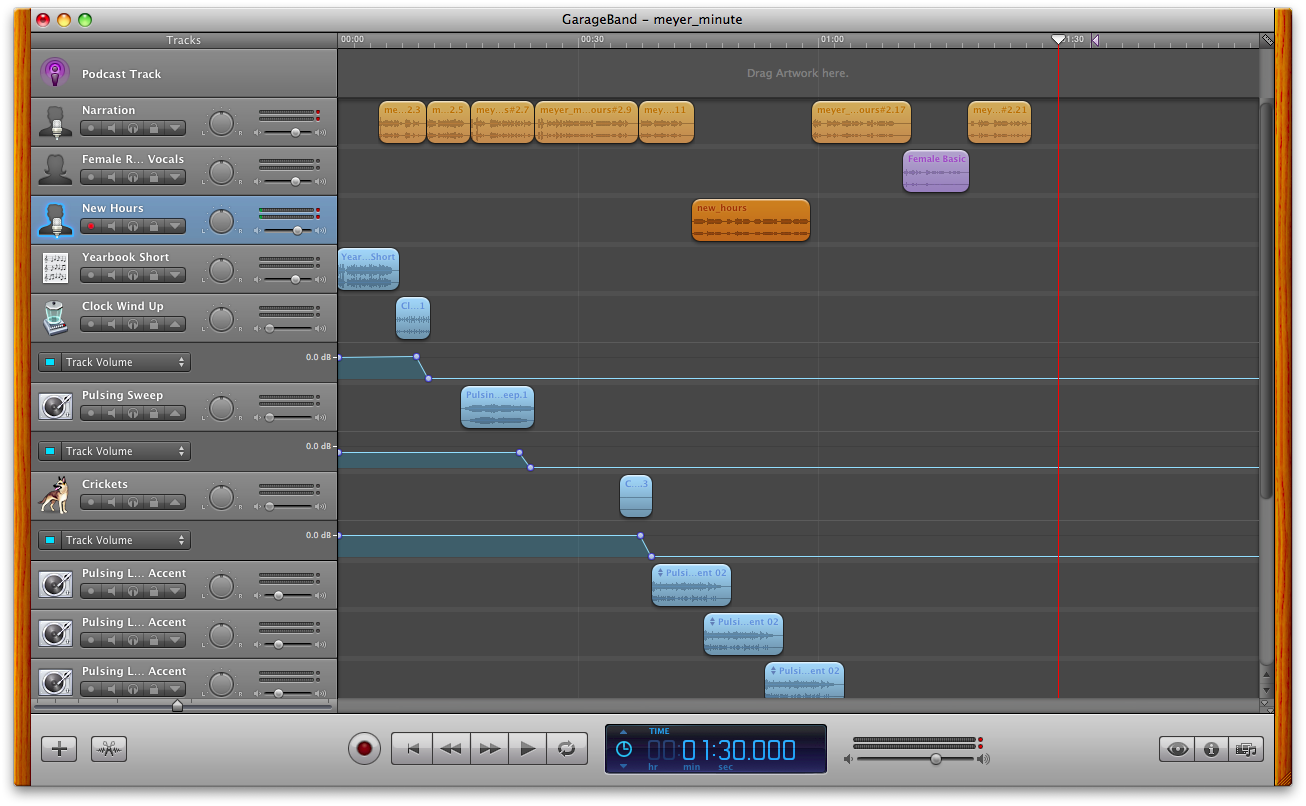
\includegraphics[width=0.75\textwidth]{img/MusicEditor.png}
   \caption{Example of music splicing software. Relevant is the time-sequence manipulation with blocks.}
   \label{img:MusicEditor}
\end{figure}


\subsubsection{Rough UI Concept}

\textit{See Figure \ref{img:AppConcept}}

\begin{figure}[ht]
   \centering
   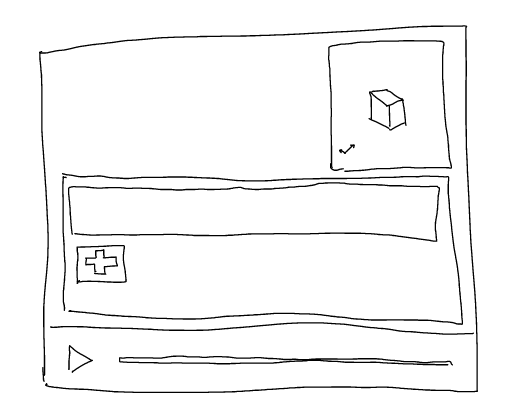
\includegraphics[width=0.75\textwidth]{img/AppConcept.png}
   \caption{First drawing for the design of the application UI.}
   \label{img:AppConcept}
\end{figure}

\subsection{Communications Specifications}

It is straightforward that communication between cubli and choreographer is necessary in order to put choreographies into action. However, the exact implementation of these communications is not, itself, obvious.\\

The observed particularities of this mode of UART transmission are described as follows:
\begin{itemize}
\item communications involve the transmission of 8-bit "packets" ( or "characters" ) in sequence
\item all devices share the same frequency channel. i.e, when a device sends a packet all other devices immediately receive it
\item the packets themselves are not signed or identified
\item there is a significant probability of a cubli failing to receive a packet, or receiving packets in the wrong order
\item there is a much lower probability of the computer failing to receive a packet
\end{itemize}

Identification, verification, and disambiguation of messages, if necessary, have to be implemented within these constraints.\\

Identification: In a scenario where only one cubli and computer communicate, it would be possible to forego the encoding of sender and recipient inside messages, as they are implied in one-on-one conversation. However, since the goal of this project is to have a choreographer functioning with several cublis simultaneously it becomes necessary for communications to explicit the devices from which they are emitted and to which they are intended.\\

There would be several ways to implement this, notably at the packet level - for example, using some bits from each packet to encode the sender - or at the message level - each group of chunks containing a header with the relevant information.\\

The principal advantage of the first method is that it enables the removal of transmission failures in the case of simultaneous emission, as it allows identification of packets in any situation. In simpler terms, for example if two packet sequences are sent simultaneously by two devices: the orginal sequences can still be disambiguated by organizing packets based on the senders - which are encrypted in every byte - and the garbled messages can thus be reassembled.\\

However, it also means that the more devices a protocol accepts, the lower the amount of information available in each packet for data itself. For example, if a maximum of 10 devices can be connected at once, 3 bits of every byte must now be dedicated to identification metadata, which leaves 5 bits for data: instead of 255 possible values p. packet, we now have 32. This is disadvantageous as the amount of "wasted" space does not decrease as the message size increases, when using this method.\\

\begin{figure}[ht]
   \centering
   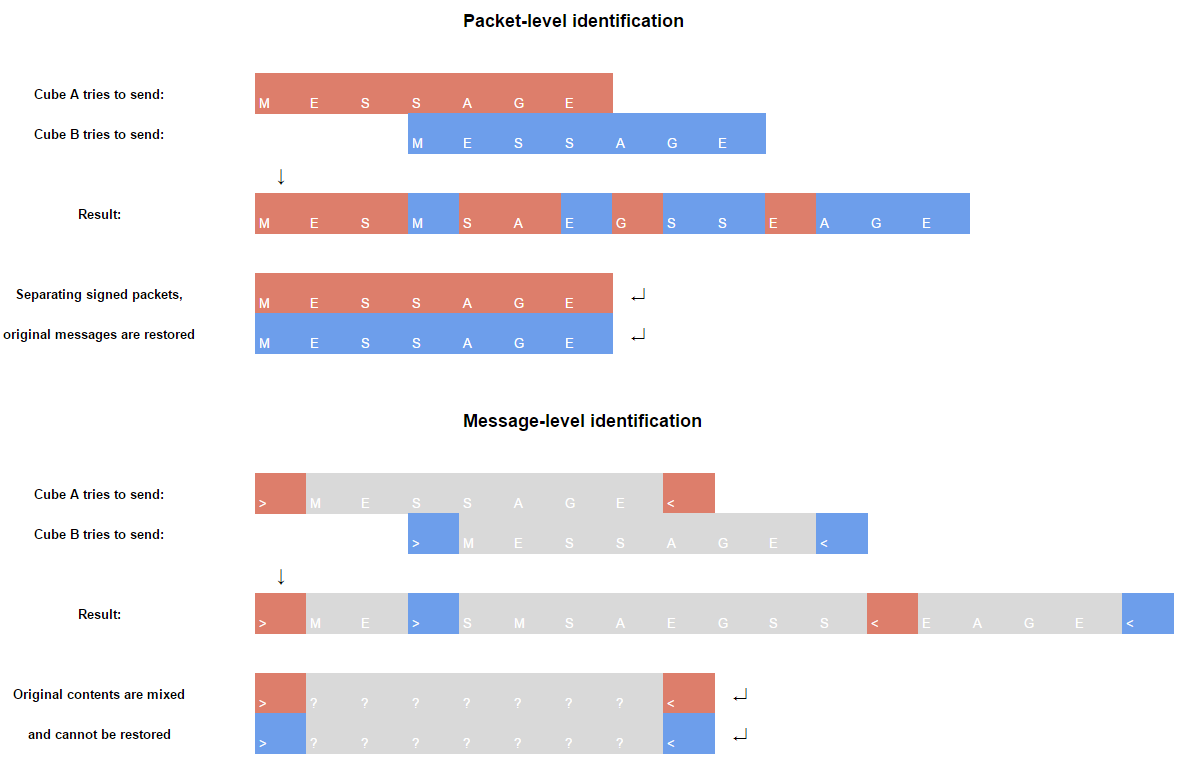
\includegraphics[width=1\textwidth]{img/disambiguation.png}
   \caption{Recovering mixed-together messages with packet-level or message-level sender identification.}
   \label{img:disambiguation}
\end{figure}

It follows that the second method is preferable where the risk of simultaneous message emission is relatively low. We see later that this is indeed the case here. \\


Verification: Does this project require that the integrity of messages be verified? For any scenario where the rate of successful transmission can be expected to be lower than 100\%, ensuring that messages are emitted and received as intended is essential. In addition, though it requires extra effort during development, the necessary overhead to verify message contents during operation is low enough that it would be reasonable to implement it here even if a transfer rate close to 100\% was expected.


\subsection{Cubli Specifications}

The purpose of this project is to add new behavior to Cubli, without removing that which already exists. That is, one of the main goals is to preserve all original functionality.

As such, it is necessary to create a state for cubli in which it performs choreographies. This is distinct from another, "standard" state, in which cubli behaves as it previously did.

The former, called "choreography" state, should be entered at the start of the performance and exited at the end.

In addition, it is expected that at least one new basic move will have to be implemented in order for cubli to be able to perform sequential moves without assistance: jumping back down from an edge to a face, and from a corner to a face.

\subsubsection{Choreography State}

In the choreography state, a cubli should keep track of the elapsed choreography time, and execute the action corresponding to the current time.\\

Synchronized choreography movements between cublis is a desired feature, though not a necessary one. It is more important that the implementation of this synchronization does not get in the way of more essential features.\\

\section{Failure Scenarios \& Responses}
This section discusses the planning of failure estimation and handling.
\textit{What could go wrong, and what cubli should do if it does}.\\

As in every complex system, there are certain and uncertain likelihoods of something going wrong at any stage and for a multitude of reasons.\\

In this section we attempt to identify the most important failures which can affect any step of choreography, and come up with appropriate responses. These responses shape the entire project execution in no small way.\\

Here, failure importance is considered in the risk-analysis sense. That is, it is based on two factors: probability of occurrence, and severity of the disruption. Disruption is the amount of deviation from expected behavior, weighed by subjective preference for avoiding the resulting erroneous behavior. \\

Regarding the usefulness of this section:\\

Of the two factors taken into account above, the second, that is the disruptions themselves, can in many cases be deduced logically ( "if A fails, then B fails. If both fail, X will not be fulfilled" ), though it generally still contains probabilistic unknowns. The first factor, probability of occurrence, has to be at first intuitively gauged, since at the outset very little is known about hardware and software reliabilities, and only later measured.\\

For this reason, failures can at the start be incorrectly evaluated, their consequences or the responses misunderstood, or even simply not expected. As the project progresses, the actual importance of failures - through both factors - becomes gradually clearer.  This evolution leads to modification of the planned implementation in order to account for these corrections.

\subsection{User Input Error Handling}

A hard to predict mode of errors in a human-controlled environment are nonsensical inputs which can occur when the user makes a mistake, or the interface leads to misunderstanding - for example if it is not designed optimally.\\ 

One aspect of an system is its tolerance to unrecognized/illrecognized inputs, and how strictly it attempts to prevent them from occuring, or corrects them. In this project: the aim was for the limits of possible interactions to be intuitively clear to the user. Contradiction to the user's commands must be avoided, and in the event of incoherent input, if a correction is to be made it should be the smallest correction leading to acceptable behavior. In addition it must be accompanied by a notification of this correction, communicated to the user in a non-intrusive way.\\

This philosophy can be understood in practice. For example, in the implementation of choreography completion, which defines how the application adds "missing" moves when the user places together actions that can not rationally follow one another.



\subsection{Communication Failure Handling}

At the outset, the probability of occurence for such failures was expected to be low, yet not insignificant. As for the disruption caused by this event, it should vary based on the situation in which it occurs ( for example at a time-critical moment of the choreography, a failed transmission can have a much greater impact on the performance ), and the accumulation of communication errors.

If several messages in a row fail to reach their recipients, the deviation from desired behavior can widen critically.\\

The response to this issue must be proportionate to the risk they cause, and since very little is known at the start regarding actual message delivery rates, the various scenarios are all to be considered.\\

If messages are rarely, if ever dropped, chances of several messages being dropped in a row become negligible. In such a scenario, communication protocols which perform a single check, or no check ( messages are assumed as delivered unless notified otherwise ), are sufficient in nearly all cases. Extra measures are not immediately necessary.\\

When messages have a significant probability of being dropped, and the same applies to errors occuring several times in a row, the communication protocol must become increasingly complex to ensure that resulting behavior is still reasonable. Each message must be sent over and over until a confirmation is received, and it should also be expected that confirmations have to be sent several times in case they are also dropped. Timeout delays must be introduced, to ensure that every back-and-forth exchange has a chance to complete.\\

As the probability of failure increases, it becomes increasingly likely that back-and-forth exchanges of information are unable to complete in reasonable time. Communications must also be reduced to a minimum, which can mean significant changes in the organisation of devices.\\

The actual protocols which were developed for this project are detailed in the next chapter.

\subsection{Cubli Failure Handling}

Cubli's ability to learn and perform movements is impressive and works very well. It still happens that moves fail with varying likelihoods - especially difficult moves. This is the principal source of failure in a choreography.

Thus, it is expected that this mode of failure has both a significant probability of occurence, and unarguable ability to disrupt the intended execution of a choreography.\\

As such, the strategy for recovering from and reacting to failed moves is important, and though in any case the perfect execution of the choreography is lost when such a failure happens, different recovery methods work to salvage different aspects of the remaining choreography execution.

\subsubsection{Affected Cubli Recovery}

When possible, Cubli should recover by itself. This is generally the case when an attempt to jump to an edge, for exampleHowever, in Cubli's current development state, there are positions from which the possibility of performing moves is not programmed, and thus in which Cubli requires outside intervention.\\

Regarding the above, ensuring Cubli's ability to move from any position is an interesting future development, also discussed in the \textit{Results \& Discussion} chapter.



\subsubsection{Other Cublis}

When one cubli fails, the choreography is generally considered as being in a Failure state. Several ways of handling this scenario are to be considered, the main factor being how all other cublis should behave when one fails.\\

A few examples of potential choreography recovery methods and their consequences:\\

\begin{description}
\item[A.] Letting unaffected cubes continue their program, without waiting. The affected cube recovers as fast as possible, and then continues its program with a delay with respect to the others.
The particularities of this strategy are as follows:

\begin{itemize}
\item[-] Sync between timelines is not preserved in case of failures
\item[+] Non-failed cubes' timelines remain true to their intended versions.
\item[+] Almost no intervention is required, and the communication cost, as well as likelihood of aggravating a failure are low.
\end{itemize}

\item[B.] Notifying all cubes in case of failure, pausing all devices until the issue is resolved, and then resuming the choreography all at once.

\begin{itemize}
\item[-] The more procedures are put in place to ensure the correct behavior of all cubes, and the exactitude of sync, the more complex this strategy, and the longer it takes before choreographies resume. 
\item[+] If done correctly, the simultaneity of all timelines is preserved, and only the length of the global choreography is increased by a failure.
\end{itemize}

\item[C.] Forgoing the failed move. Other cublis proceed unaffected, and the failed cube picks up the choreography at the next performable move.

\begin{itemize}
\item[-] It is not always possible to find a compatible move following the failed one, based on the current state of the affected cube.
\item[-] As a result the failed cube's timeline can be significantly different from the original
\item[+] No communication is necessary, and all other cubes continue unaffected
\end{itemize}

\textbf{Note:} This method in particular can lead to interesting ways of correcting failures, with solutions of varying complexity. For example, one could imagine algorithms responsible for re-shaping the remaining choreography in real-time, in order to [as quickly as possible/with the largest likelihood of success/as similarly to the intended plan/etc] have the cube get back into the groove.
Though it certainly would be an interesting avenue of experimentation, since well-executed implementation of this method reduces the need for inter-device communication, it was not necessarily the most appropriate for this project.

\item[D.] Starting over, or aborting a choreography if a failure occurs.

\begin{itemize}
\item[-] In the case that failures are somewhat frequent, choreographies will be repeated endlessly, or never reach their end.
\item[+] Strictly ensures the simultaneity of timelines, and integrity of any choreography that has completed.
\end{itemize}

\end{description}

It is thus up to the implementer to decide, based on which choreography aspects are the most important to conserve, the appropriate method. It should also be noted that each of those methods also presents several alternatives regarding implementation details, which also play a role in their resulting efficiency. These particulars are discussed in the following chapter, which delves into the details of implementation.



